\documentclass[..]{subfiles}


\begin{document}

\chapter{The Bitcoin Backbone Protocol}\label{chap:protocol}

This chapter has three main sections. In the first one a concrete instantiation of the model described in Chapter \ref{chap:model} is given. In the second section a description of the Blockchain underlying data structure is provided. Last the protocol is properly defined and parameterized. This chapter is mainly based on \cite{garay2015bitcoin}.

\section{Model Instantiation}

The following model instantiation is one chosen in order to model the conditions usually present in the settings the protocol will be executed. The decision taken try to model such conditions in the simplest, yet most concrete possible manner.

A set of parties $P$, an adversary $\mathcal{A}$, an environment $\mathcal{Z}$, a control program $C$ and a protocol $\Pi$ are considered. The total number of parties $n$ is defined from the start as well as the number of parties control by the adversary $t$. Three services, a functionality and two random oracles, need to be defined in order to model network communication, hashing power and the capacity to create random strings called \textit{nonces}:
\begin{itemize}
	\item Diffuse functionality: In order to provide better readability without loss of generality the INPUT tape of each party will be split in two: 
	\begin{itemize}
		\item Communication tape. Noted as RECEIVE. It will be used to store messages coming from other parties.
		\item Input tape. Noted as INPUT. It will be used to store messages coming from the environment $\mathcal{Z}$.
	\end{itemize}
	The diffuse functionality maintains a \textit{round} counter which is initialized at 1. The diffuse functionality acts like a buffer that stores parties messages and delivers them at the end of the communication stage: When the functionality receives an instruction to diffuse a message $m$ from a non-adversary party $P_i$ it marks the party as complete for the current round. When all parties are complete for the current round, the functionality writes all messages into the RECEIVE tape of each corresponding party. The \textit{round} counter is incremented. The adversary is excluded from this buffer mechanism, it can write messages directly in the RECEIVE tape of each party and it can fetch messages from the buffer at any point but has to send a complete message to the functionality for it to deliver honest parties messages. An illustration of the diffuse functionality can be seen in Figure \ref{fig:diffuse}.

	\item Nonce generator oracle($A(\cdot)$): The nonce generator oracles generates a \textit{unique} random string in $\{0, 1\}*$. The nonce is unique in the sense that no two calls to the nonce generator oracle return the same string. This property will be referred to as \textit{nonce entropy}. The reason for nonce entropy is discussed in Remark \ref{rem:nonce-entropy}.

	\item Hash function oracle($H(\cdot)$): This service has two modes:
	\begin{itemize}
		\item \texttt{Calculation}: When queried in calculation mode it receives an input value $x$, if $x$ has not been queried before a random value in $y \in \{0, 1\}^*$ is returned. The oracle keeps a table in which pair $(x, y)$ is stored. If the value $x$ has already been queried its pair $y$ stored in the table is returned.Every honest party $P_i$ is given $q$ calculation queries each round. The adversary $\mathcal{A}$ is given $t \cdot q$ queries each round. The environment $\mathcal{Z}$ is not given any queries.

		\item \texttt{Verification}: When queried in verification mode the oracle expects two values $x$ and $y$ and the oracle returns \texttt{true} if pair $(x, y)$ is stored on the table, otherwise \texttt{false} is returned.
	\end{itemize}
\end{itemize}


\begin{figure}
	\begin{center}
		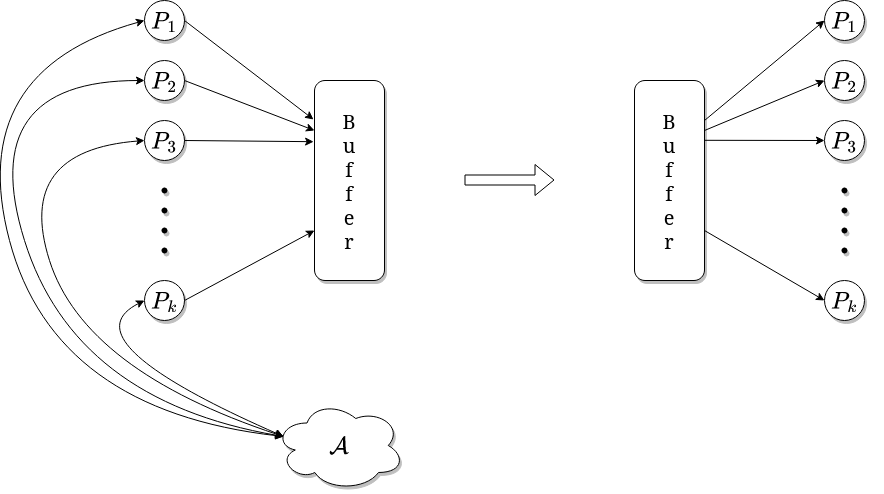
\includegraphics[width=0.95\textwidth]{figures/diffuse_diagram.png}
	\end{center}
	\caption{Diffuse functionality diagram}
	\label{fig:diffuse}
\end{figure}

The fact that parties cannot communicate directly with each other but have to make use of a diffuse functionality is an attempt to model Bitcoin't P2P network layer. The fact that the adversary can bypass the diffuse buffer by accessing any parties messages before committing theirs and writing their message directly in the RECEIVE tape is captured by saying the adversary has ``rushing''\footnotemark capabilities. On the other hand, the adversary cannot change the content of the messages sent by honest parties or prevent them from being delivered. This mimics communication over TCP/IP in the Internet in the sense that messages between parties are reliably delivered but malicious parties may change the message sender that goes through them making it appear it originates from a different source.
\footnotetext{Although the rushing capability it is strong and has some important consequences that will be stated latter it is worth saying that it is actually argued to be realistic by properly distributing malicious nodes in the network whose only task is to echo adversary messages.}

A model may be considered where not all nodes can receive all messages reliably. This can be achieved using this same model and letting the adversary control these players and simulate them honestly while not performing the \texttt{read-next-message} instruction properly at random.

The following subsection justifies there is no need to impose an strict an upper bound on the number of messages. More on Remark \ref{rem:messages_bound}.


\subsection{$q$-bounded synchronous setting}

$\{\texttt{EXEC}_{\Pi, \mathcal{A}, \mathcal{Z}}^{t, n}(z)\}_{z \in \{0, 1\}^*}$ will be used to denote the random variable ensemble that determines the output of environment $\mathcal{Z}$ for a protocol $\Pi$ that uses the services previously described: diffuse functionality, nonce generator oracle and hash generator oracle. $\{\texttt{EXEC}_{\Pi, \mathcal{A}, \mathcal{Z}}^{P_i, t, n}(z)\}_{z \in \{0, 1\}^*}$ will be used to denote the random variable ensemble describing the view of party $P_i$ after the completion of an execution with environment $\mathcal{Z}$, running protocol $\Pi$ and adversary $\mathcal{A}$. Furthermore, $\texttt{VIEW}_{\Pi, \mathcal{A}, \mathcal{Z}}^{t, n} = \cup_{i = 1,\dots,n} \langle \texttt{VIEW}_{\Pi, \mathcal{A}, \mathcal{Z}}^{P_i, t, n} \rangle$. 

Note that parties not need to be aware of the number of parties executing the protocol and, because of the unauthenticated nature of the network only protocols that do not make explicit use of the number of parties $n$ or their identities. Also note that $n$ and which parties are controlled by the adversary $\mathcal{A}$ is fixed during the execution of the protocol and they will be hard-coded in the control program $C$\footnotemark.
\footnotetext{In reality, the number of parties controlled by the adversary has to be fixed but not which ones as it is demonstrated in \cite{garay2015bitcoin}.}

Parties limited ability to produce PoWs is modeled by the limit imposed to all parties in their access to the hash function. In this model all parties computational power is supposed to be equal since all parties are given $q$ computing hash queries per round. In the real world different parties may have different computational power but this can be replicated by the model considering a parties computational power as a unit of power and having real world parties represented by clusters of one unit parties. Note that $q$ is an upper limit, it doesn't have to be reached. The reason for not giving the environment $\mathcal{Z}$ any computational power is for the adversary's computational power to be proportional to the number of parties controlled by the adversary. Thus, the environment can still help the adversary and the invested resources can be distributed in case the same hashing function is being used by another protocol running in parallel but computational power is still tied to the number of parties controlled by the adversary.


\subsection{Protocol Properties}

Theorems will be related to \textit{properties} of protocols in the $q$-bounded synchronous setting. Properties will be defined as predicates over the random variable ensemble \texttt{EXEC$_{\Pi, \mathcal{A}, \mathcal{Z}}^{t, n}$} restricting it to adversaries $\mathcal{A}$ and environment $\mathcal{Z}$ that are polynomially bounded. Such predicates will verify with high probability on $\kappa$. The probability space is determined by the choices of the random oracles of all ITMs.

\begin{definition}
	\normalfont
	Given a predicate $Q$ and fixed $q, t, n \in \N$ with $t < n$, \textit{protocol $\Pi$ satisfies property $Q$ in the $q$-bounded setting for $n$ parties assuming the number of corruptions is bounded by t} if, for all polynomial-time $\mathcal{A,Z}$ the probability that $Q(\texttt{EXEC}_{\Pi, \mathcal{A}, \mathcal{Z}}^{P_i, t, n})$ is false is negligible in $\kappa$.
\end{definition}

\begin{definition}[Negligible function]
	\normalfont
	A \textit{negligible function} is a function $F:\N \rightarrow \R$ such that, for every positive integer $c$ there exists an integer $n_c$ such that $|\mu(x)| < \frac{1}{x^c}, \ \forall x > n_c$.
\end{definition}

Intuitively a function is negligible when it is \textit{eventually} smaller than the inverse of $c$ power function(could be extended to a polynomial of grade $c$) which means it decreases faster than the $c$ power function grows. This notion is very common in cryptography and is strictly linked to the definition of continuous function, is allows to claim that error probability decreases ``very'' fast. To simplify the discussion $z$ in $\{\texttt{EXEC}_{\Pi, \mathcal{A}, \mathcal{Z}}^{P, t, n}(z)\}_{z \in \{0, 1\}^*}$ will be fixed to $1^\kappa$. Therefore, the whole security analysis depends on $\kappa$ and it will be the known as the \textit{security parameter}. Note that the number of parties controlled by the adversary $t$ and the total number of parties in the system also have a huge impact on the security analysis but they are not a parameter since they can't be change by the protocol. 

\begin{remark}\label{rem:messages_bound}
	\normalfont
	Because computational resources are bounded there is no need to impose an upper bound on messages since sending messages means spending computational resources, thus it provides no advantage and the adversary has no way to turn this in its favor.
\end{remark}



\section{Blockchain Definition}

Let $H(\cdot)$ be a cryptographic hash function with output $\{0,1\}^\kappa$. A \textit{block} is a triple $B = \langle \alpha, \rho, x \rangle$. A block will said to be valid if it that satisfies predicate $\texttt{validblock}^T(B)$ defined as:
$$H(\alpha, \rho, x) < T$$
Where:
\begin{itemize}
	\item $\alpha \in \N$, represents a \textit{nonce}. It will be used to generate different inputs for the hash function in order to obtain a combination that satisfies $\texttt{validblock}^T(B)$ once $\rho$ and $x$ are fixed.

	\item $\rho \in \{0,1\}^\kappa$, represents a hash reference to the previous block. It will be used in order to ensure the computational efforts needed to extend a block called PoW cannot be used at the same time to compute more blocks.

	\item $x \in \{0,1\}^*$, represents the \textit{content} of the block.

	\item $\N \ni T<2^\kappa$, represents the \textit{difficulty level}. This value may change across different blocks in order to adjust the rate at which new blocks are produced. This is useful in order to maintain an steady mining rate in case the number of parties may change between rounds.
\end{itemize}

A \textit{Blockchain} or a \textit{chain} is a tuple of blocks $\C = \langle B_1, \dots, B_n \rangle$. By convention the empty tuple $\epsilon$ is also a chain. The length of a chain $C$ is its number of blocks and is noted by len($C$). By convention len($\epsilon$)$= 0$. Given a chain $C$ with len($C$)$ = n > 0$, its \textit{content}  is defined as a n-tupla $x_{\C} = \langle x_1,\dots, x_n \rangle$ where $x_i$ represents the $x$-values of block $B_i$ in chain $C$. The last block of a chain $C$ is called the \textit{head} of the chain is noted head($\C$). By convention head($\epsilon$) $= \epsilon$, the empty block.

Given a chain $\C = \langle B_1, \dots, B_m \rangle$ and $k \in \N$, let $\C^{\lceil k} = \langle B_1, \dots, B_{m-k}\rangle$, i.e, the chain resulting from erasing the last $k$ blocks from $\C$. If $k \ge m$ then $\C^{\lceil k} = \epsilon$ by convention. Also, given two chains $\C_1, \C_2$ it will be said $\C_1$ is a prefix of $C_2$ if exists $k \in \N$ such that $C_2^{\lceil k} = C_1$.

A chain $\C$ with head($\C$) = $\langle \hat\alpha, \hat\rho, \hat x \rangle$ may be extended by appending a block $B = \langle \alpha, \rho, x \rangle$  such that $\rho = H(\hat\alpha, \hat\rho, \hat x)$. This condition is known as proof of work and abbreviated as PoW. Only a block with $\rho = 0$ can extend an empty chain $\epsilon$\footnotemark. A chain $C$ extended by block $B$ it is noted as $\C_{new} = CB$ and verifies head($\C_{new}$)$=B$.
\footnotetext{The first block of a chain is called the Genesis block. It doesn't point to any other block and it usually contains some trusted setup information hard-coded in the source of the application. In the original Bitcoin protocol the Genesis block, among other information, contains the following sentence: ``The Times 03/Jan/2009 Chancellor on brink of second bailout for banks'' which is the main headline of The Times issue of such date. The quote has two purposes, in the first place, it demonstrate the block was mined after such date and, secondly, it points at the financial instability as a likely cause for the Bitcoin development.}

\begin{figure}
	\begin{center}
		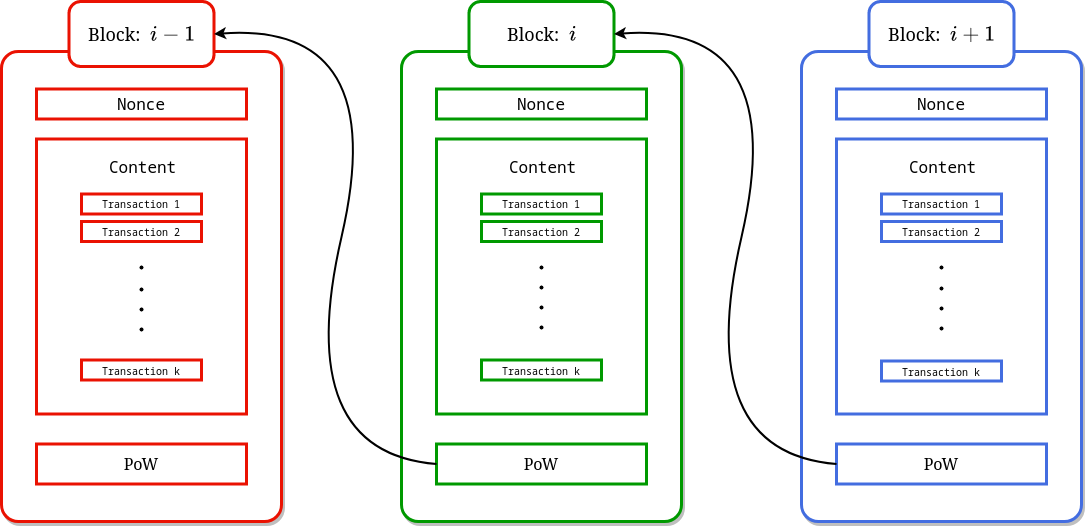
\includegraphics[width=0.95\textwidth]{figures/blockchain.png}
	\end{center}
	\caption{Blockchain sketch}
	\label{fig:blockchain}
\end{figure}


\begin{remark}
	\normalfont
	$\rho$ is a hash value, thus, given a block $B$ there is no way to know which block precedes $B$ it is also given as a chain in which case it can be checked the blocks are properly ``linked''.
\end{remark}



\section{Protocol Definition}

\subsection{External Functions}

The external functions are:
\begin{itemize}
	\item Content validation predicate $V(\cdot)$: Given a chain $\C$ the content validation predicate receives $x_\C$ as input and returns 1 if the content is consistent with the application built on top of the protocol. Otherwise 0 is returned. By convention $V(\epsilon) = 1$.

	\item Input contribution functionality $I(\cdot)$: The input contribution function receives tuple ${\langle \C, \textrm{INPUT}(), \textrm{RECEIVE}() \rangle}$ as input, where $C$ is a chain, INPUT$()$ are the contents of the input tape and RECEIVE$()$ the contents of the network tape. The function will produce some block content $x$ . The purpose of $x$ is to be used in the making of a block that extends $\C$, thus, it is sensible to ask for $x$ to be consistent with the content of $\C$, i.e, for any chain $\C$ with $x_\C = \langle x_1, \dots, x_n \rangle$ a value $x$ produced by $I(\C, \cdot, \cdot)$ must satisfy $V(\langle x_1, \dots, x_n, x \rangle) = 1$. It is important to note that this functionality can preserve state in the form of a table or any other structure that may be used in any other future invocation.

	\item Chain reading function $R(\cdot)$: The chain reading function receives a chain $C$ as input and generates some kind of output dependent on the purpose of the application built on top of the protocol. In its simplest form this function returns the chain's contents. The importance of the existence of this function can be debated. In the protocols described in Chapter \ref{chap:applications} this function is quiet simple and only uses information relative to the chain's contents but it doesn't have to be the case. In case information related to the chain other than its content is needed in order to create an output then the chain's content will not be enough and this function's existence is mandatory.
\end{itemize}

\begin{figure}
	\begin{center}
		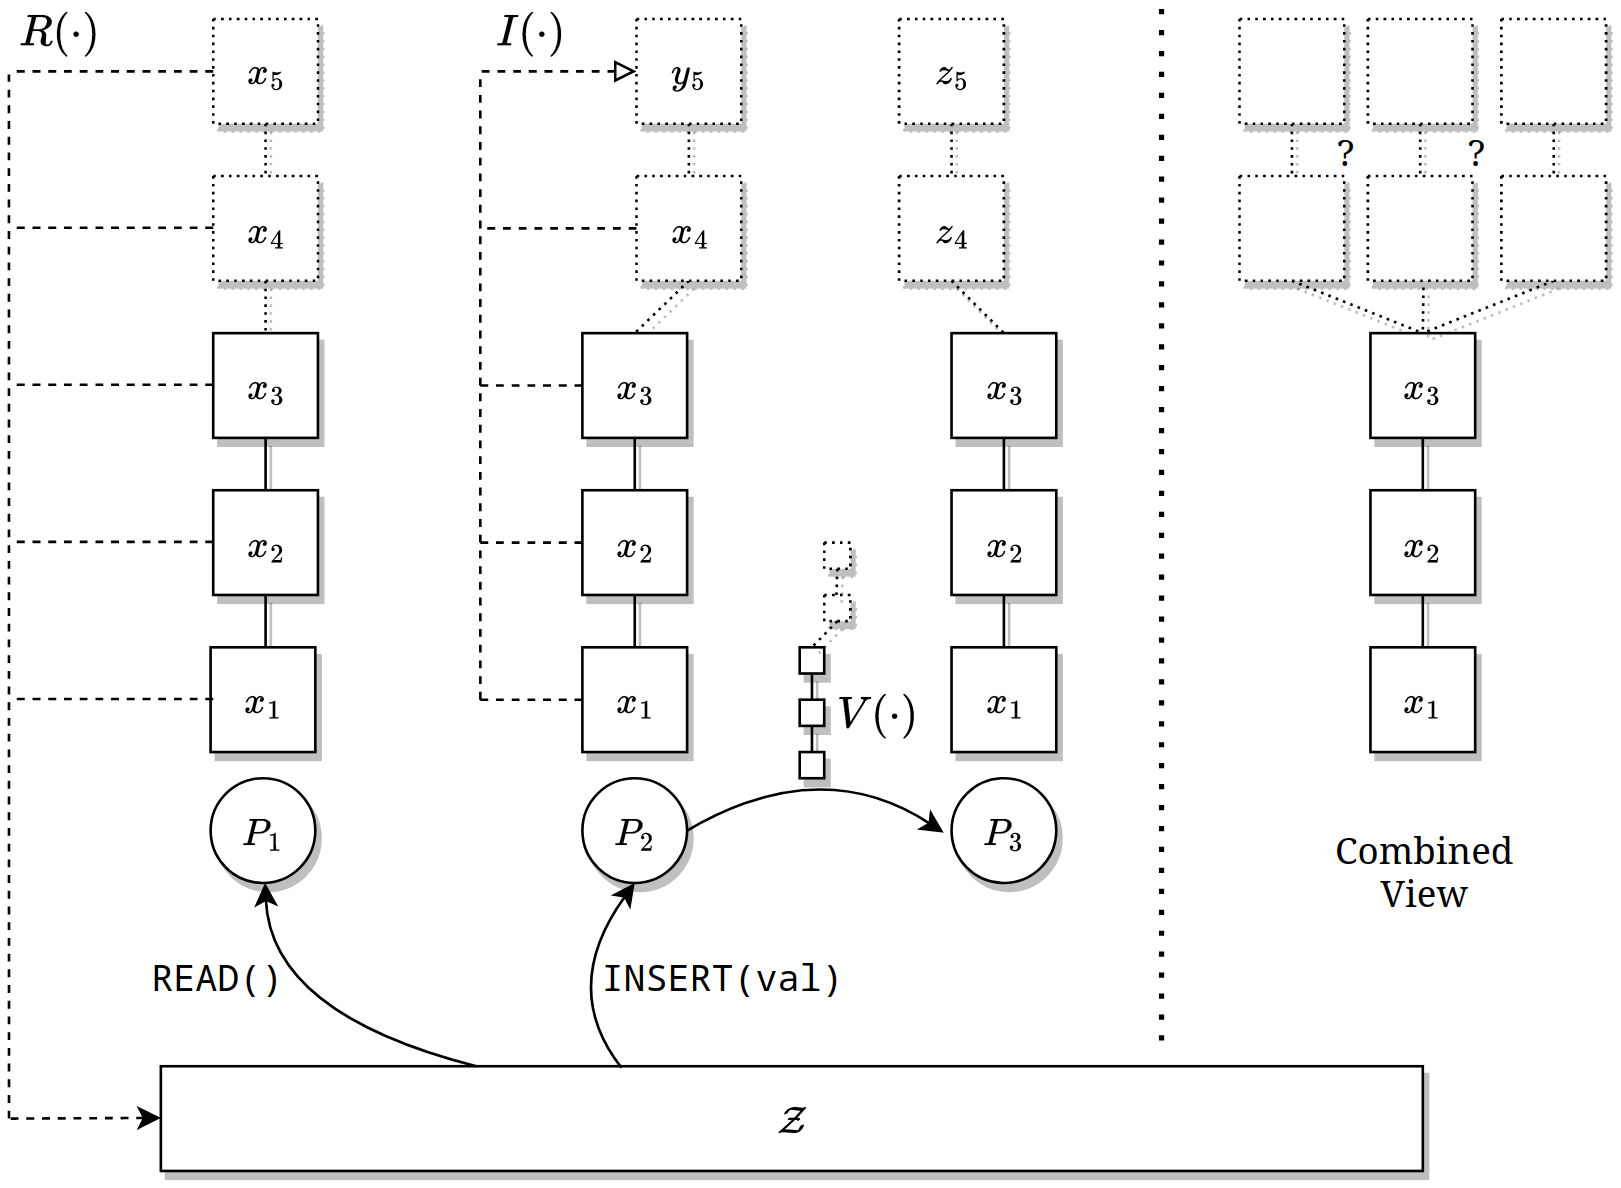
\includegraphics[width=0.95\textwidth]{figures/example.png}
	\end{center}
	\caption{Overview of basic operations}
	\label{fig:example}
\end{figure}

In Figure \ref{fig:example} the basic operations of the bitcoin backbone are illustrated. Party $P_1$ receives READ instruction from the environment $\mathcal{Z}$ that resolves returning the value output by function $R(\cdot)$ which is the sequence $\langle x_1, \dots, x_5 \rangle$. Party $P_2$ receives instruction INSERT value $val$ which resolves calling functionality $I(\cdot)$ in order to produce some valid content $y_5$ to extend its current chain. It calculates a new block successfully and, after appending it to its current chain, the resulting chain is broadcast. Party $P_3$ receives the chain calculated by $P_2$ and proceeds to check its content via the content validation predicate and its correct structure. If the chain is correct it will need to decide on which chain to keep. Last, note that the combined view of parties $P_1, P_2, P_3$ is inconsistent but they agree on a common prefix $\langle x_1, x_2, x_3 \rangle$.

\subsection{Auxiliary Algorithms}

Three algorithms will be necessary in order to build the protocol:

\paragraph{Chain validation.} The algorithm called \texttt{validate\_chain} performs a validation of the structural properties of a chain. It takes a chain $C$, the value $T$ and a hash function $H(\cdot)$ as input. It is parameterized by the validation predicate $V(\cdot)$. The algorithm verifies every blocks in $C$ is valid by checking it fulfills the $validblock^T$ predicate and also verifies every block extends the previous one by certifying its PoW. If all blocks are verified and their content is consistent, i.e, $V(x_\C) = 1$, the chain is deemed as valid, and the algorithm returns 1. Otherwise the chain is rejected and the algorithm returns 0. Its pseudocode is represented in Algorithm \ref{validate}.

\begin{algorithm}
	\caption{\textit{Chain validation predicate} algorithm. Parameters are $T$, the cryptographic hash function $H(\cdot)$ and the content validation predicate $V(\cdot)$. Input is $\C$.}\label{validate}
\begin{algorithmic}[1]
	\Function{\texttt{validate}}{$\C$}
	\If{$\C = \epsilon$}
		\State \Return True
	\EndIf
	\State

	\If{$V(x_\C)$}
		\State $B \gets$ head($\C$)
		\State $\rho \gets H$($B$)
		\Repeat 
			\State $\C \gets \C^{\lceil 1}$
			\State $B' \gets$ head($\C$)
			\State $\rho' \gets H$($B'$)
			\If{$(\texttt{validblock}^T(B) = \textrm{False}) \lor (\rho \neq \rho')$}
				\State \Return False
			\EndIf
			\State $\rho \gets \rho'$
			\State $B \gets B'$
		\Until{($\C = \epsilon$)}
	\EndIf
	\State
	\Return True
	\EndFunction
\end{algorithmic}
\end{algorithm}


\paragraph{Chain comparison.} The second algorithm is called \texttt{maxvalid} it utilizes \texttt{validate\_chain} and its purpose is to select the ``best'' chain out of a set of chains. The algorithm iterates on the set of chains comparing them by pairs using the function \texttt{max} which encodes some kind of order in the space of chains. The main factor used by function \texttt{max} in order to determine the best chain is the length. When two chains have the same length some tie breaking criteria needs to be applied. There are many options but the one chosen will be to always return the first chain. Since the set of chains is ordered by arrival time, this rule means any party will prefer its local chain opposed to any other chain. This is consistent with the current Bitcoin operation. Since solving PoW takes computational power the longest chain criteria means parties are always looking forward to obtain(and thus extend) the current longest chain which is the one that amasses the most computational power. This characteristic will be key in the following analysis. The algorithm's pseudocode can be seen in Algorithm \ref{maxvalid}.

\begin{algorithm}
	\caption{\textit{Chain comparison} algorithm. Parameters is \texttt{max($\cdot$)}. Input is $\{\C_1, \dots, \C_k\}$.}\label{maxvalid}
\begin{algorithmic}[1]
	\Function{\texttt{maxvalid}}{$\{\C_1, \dots, \C_k\}$}
	\State aux $\gets \epsilon$
	\For{i=1: k}
		\If{\texttt{validate}($\C_i$)}
			aux $\gets $ max($\C_i$, aux)
		\EndIf
	\EndFor
	\State
	\Return aux
	\EndFunction
\end{algorithmic}
\end{algorithm}


\paragraph{Proof of Work.} The purpose of the third algorithm referred as \texttt{pow} obtain a block such that verifies the PoW condition. The algorithm takes some content value $x$ and a chain $C$ as input. It is parameterized by the values $q$ and $T$ and a cryptographic hash function $H(\cdot)$ and the functionality $A(\cdot)$. The algorithm will use functionality $A(\cdot)$ in order to generate up to $q$ random nonces to which it will append input $x$ as well as the hash identifier of the current head of the chain to build a valid block which accomplishes PoW. If one of the $q$ trials is successful the chain extended with the calculated block is returned; otherwise the current chain is returned. The algorithm is illustrated in Algorithm \ref{pow}.

\begin{algorithm}
	\caption{\textit{Proof of work} algorithm. Parameters are $q$, $T$, a cryptographic hash function $H(\cdot)$ and the nonce generator functionality $N(\cdot)$. Input is ($\C, x$).}\label{pow}
\begin{algorithmic}[1]
	\Function{\texttt{pow}}{$\C, x$}
	\If{$\C = \epsilon$}
		\State $\rho \gets 0$
	\Else
		\State $\rho \gets $ $H$(head($\C$))
	\EndIf
	\State

	\For{i=1: q}
		\State $\alpha \gets A()$
		\If{$H(\langle \alpha, \rho, x \rangle) < T$}
			\State $B \gets \langle \alpha, \rho, x \rangle$
			\State $\C \gets \C B$
			\State \textbf{break}
		\EndIf
	\EndFor
	\State
	\Return $\C$
	\EndFunction
\end{algorithmic}
\end{algorithm}

\begin{remark}\label{rem:nonce-entropy}
	\normalfont
	If two parties could obtain the same PoW then the adversary $\mathcal{A}$ could have and advantage since they could share their history of hashed values constantly and this could give them the upper hand in calculating PoWs since honest nodes could spend their hash queries in exactly the same values. Obviously this is not very relevant and the probability of such event decreases exponentially in $\kappa$, still, the nonce entropy hypothesis is not too strong and it greatly simplifies the discussion.
\end{remark}


\begin{remark}
	\normalfont
	The adversary cannot ask for help in the calculation of PoW to an external process since the state of the hash calculation oracle cannot be replicated in any way. Also note that this is not restrictive since there additional computational power can be modeled by increasing $t$ value.
\end{remark} 




\subsection{The Backbone Protocol}

Now the Bitcoin backbone protocol will be described using the functions described previously. The protocol receives no input. The protocol is parameterized by two functions, the input contribution function $V(\cdot)$ and the chain reading function $R(\cdot)$. The first step is to initialize the variables. Then an ``infinite'' loop is executed although the following analysis is only valid in case the total polynomial time is polynomial in $\kappa$(as it has been already stated). The loop has two main sections.

In the first section, the best valid chain $\C$ is selected between its local chain and the ones available in the communication tape RECEIVE$()$ using function \texttt{maxvalid}, the other chains are discarded. Some block content $x$ is created invoking functionality $I(\cdot)$ over the current chain. Note that, as stated before, functionality $I(\cdot)$ may use any kind of knowledge about the state of the execution and the contents of the communication tape RECEIVE$()$ and the input tape INPUT$()$. Then, the party executing the protocol attempts to extend its chain $\C$ with content $x$ calling \texttt{pow} function. If $\C$ is successfully extended the resulting chain is broadcast using functionality DIFFUSE$()$, otherwise an end of round signal is issued(represented by a termination message $\perp$).

In the second section, if the input tape INPUT$()$ contains value READ the output of function $R(\cdot)$ over the current chain $\C$ are written in the OUTPUT$()$ tape. Finally round counter is increased.

Two clarifications are worth doing. Although the protocol is executed indefinitely the incoming analysis only applies when the total running time is polynomial in $\kappa$. In this particular version of the protocol only two types of entries expected in the input tape: (INSERT, $value$) and READ; other inputs are ignored.


\begin{algorithm}
	\caption{\textit{Bitcoin backbone} protocol. Parameters are the input contribution function $I(\cdot)$ and the chain reading function $R(\cdot)$. Input is none.}\label{backbone}
\begin{algorithmic}[1]
	\Function{\texttt{protocol}}{}
	\State $\C \gets \epsilon$
	\State $round \gets 1$

	\State 
	\While{True}
		\State $\C \gets \texttt{maxvalid}(\C, \textrm{chains in RECEIVE$()$})$
		\State $x \gets I(\C, \textrm{INPUT}(), \textrm{RECEIVE}())$
		\State $\hat\C \gets$ pow$(\C, x)$
		\If{$\C \neq \hat\C$}
			\State $\C \gets \hat\C$
			\State DIFFUSE($\C$)
		\Else
			\State DIFFUSE($\perp$)
		\EndIf

	\State
	\If{INPUT() contains READ}
		\State \textbf{write} $R(\C)$ to OUTPUT$()$
	\EndIf

	\State
	\State $round \gets round + 1$
	\EndWhile
	\EndFunction
\end{algorithmic}
\end{algorithm}



\end{document}
